% !Mode::"Tex:UTF-8"

\documentclass[a4paper]{article}
\usepackage{ctex}
\usepackage{amssymb}    %使用宏包{美国数学协会符号}
\usepackage{amsmath}
\usepackage{multirow}
\usepackage{tabularx}
% 插图包,两个图并排
\usepackage{graphicx}
\usepackage{subfigure}

\date{} % 这一行用来去掉默认的日期显示
\title{Rapid Discrimination of apple essence base on PCA-CCH-SVM  }
\author{Jun Liu,Tiejun Pan}


% 页面设置
\usepackage[top=2.54cm,bottom=2.54cm,left=3.18cm,right=3.18cm]{geometry}
% 页眉页脚设置
\usepackage{fancyhdr}
%\pagestyle{fancy}
%\chead{\thesection}
\cfoot{\thepage}


\begin{document}
\maketitle

An important aspect of rapid discrimination of apple essences based on pattern recognition is how to use new training data to improve the accuracy and control the training time. In this paper,PCA-CCH-SVM method and Raman spectra were used in combination for fast discrimination of apple essences from different manufactories.PCA-CCH-SVM built on a convex hull of support vectors and new Raman spectra data to classify the apple essence based on features obtained from Raman spectra. The classification model have been evaluated with 10-fold cross validation. The results from this study demonstrated that our approach has good classification accuracy while the training is significantly faster than normal SVM classifiers.

Key words: Apple Essences; Convex-Concave Hull vector; PCA-CCH-SVM; rapid discrimination

%=============第一部分 简介===================
\section{Introduction}
    % 苹果香精检测的背景、
Apple essences are widely used as a food additive in food industry. Rapid identification of apple essence for the quality control of food industry is of great significant. Apple essence is a complex mixture of a large number of volatile compounds $^{\cite{Sanz et al.}}$. Usually the detection of apple essence is carried out by chemistry-based methods and sensory evaluation. Sensory evaluation is a traditional and most commonly used method, but its accuracy and objectivity cannot always be ensured because sensory evaluation staff’s judgement can be affected by their health condition, emotions, and the environment. Chemistry-based methods such as gas chromatography,  mass spectrometry, and gas chromatography-mass spectrometry are highly reliable because they use a complete component-by-component approach. However, their shortcomings include excessive test items, being time-consuming, complicated operation, and low capability for insitu and rapid measurements $^{\cite{K.P. Bennett1}}$ $^{\cite{K.P. Bennett2}}$. Overall, developing a novel, rapid and reliable method to identify  essence is of positive significance.

Raman spectroscopy is a technique which is arising from inelastic scattering of laser light by the molecular vibration inside the sample. As a result, the scattered photons are emitted with the different frequency or energy. This difference in frequency between incident and emitted protons provides finger print about the rotational, vibrational and other low frequency transitions in molecule. Thus Raman spectrum, which is the plot of intensity as function of Raman shift, is a rapid detection method developed in recent years, with fast, efficient, non-polluting, without pre-treatment, lossless analysis, etc., and are been widely used in many areas. $^{\cite{Zhou Xiu jun}}$
$^{\cite{WANG Jun}}$ $^{\cite{SHA Min}}$.

Support Vector Machine (SVM) $^{\cite{Vapnik}}$ has been successfully used for data mining, pattern recognition and artificial intelligence fields [2–5]. With labeled data, SVM learns a boundary (i.e., hyperplane) separating different class data with maximum margin.
The classification process usually face the new evolving data, the initial training sample set can not reflect all the sample information. When new training samples are accumulated to a certain scale, in order to obtain the new sample information,it would like to integrate these examples and train a new classification model.However, the training of a SVM has the time complexity of $O(M^3)$(M is the number of training samples), it does benefit large-scale online applications$^{\cite{Stefan}}$ $^{\cite{Asdrúbal López Chau et al.}}$ $^{\cite{XIAORong}}$.

It is noteworthy that performance of classification method for apple essence is evaluated not only based on accuracy, but also the rapidity, which are also of great significance in practical applications. To attack this problem,lots of works have been done. One way is to reduce training samples with a certain sample selection strategy. The quality of training data set is vital to the performance of the classifier being constructed. Syed et al.$ ^{\cite{Stefan}}$ $ ^{\cite{{K.P. Bennett1}}}$ worked out an incremental algorithm based on SVM, which retains only the support vector set as a historical training sample.

The main contribution of this paper is that a novel hybrid classification method based on Principal Components analysis (PCA) and Convex-Concave-Hull Support Vector Machine (CCH-SVM), combined with Raman spectra is proposed.Experimental results indicated that PCA-CCH-SVM, as a classifier,was tested in terms of classification rate and running time.Compared with normal SVM,PCA-CCH-SVM can run much faster with similar accuracy rate. Experimental results showed that PCA-CCH-SVM combined with Raman spectra can be a rapid, accurate  method for classification of apple essences.

%=============第二部分 实验与材料===================
\section{Experiments and Materials}
\subsection{Sample collection and preparation}

Three brands of apple essence samples were purchased from three famous flavors and fragrances companies in China. Three batches of each brand and  each batch of 10 samples were collected. Apple essence contains a large number of volatile, low content components.The complex pretreatment methods of samples have some impact on these components.In order to avoid introducing other impurities or the distortion of component proportion caused by improper pretreatment method,in this experiment, the test samples are prepared by high dilution of pure water. Apple essence was respectively diluted 10 times and 1000 times with high purity water in the volumetric flask.The  standard  safety  rules  have  been  followed  at  each step from sample collection till acquisition of Raman spectra.For each sample, we collect 10 Raman spectra at different times. In total, 900 Raman spectra were achieved.


\subsection{Raman spectrum acquisition}%拉曼光谱的获得
Raman spectrum for all samples have been acquired with Raman spectrometer ( Prott-ezRaman-d3,Enwave Optronics, USA ).Raman  signal  is  normally  very  weak  as  compared  to  Rayleigh  scattering,  therefore  an acquisition time of 10 seconds has been used for recording each spectrum.The spectrum from the  samples  have  been  recorded  in  the  spectral  range  of  250 $cm^{−1}$  to  2350 $cm^{−1}$,  as  it contained the most useful information.

\subsection{Data preprocessing}%
In this study, we used PCA to remove redundant features and several previous principal components were extracted as the inputs of the classifier for apple essences.
PCA is  a  method  for  the  re-expressing  multivariate  data. It  allows  the researcher to reorient the data so that the first few dimensions account for as much  of  the  available  information  as  possible.  The  principal  components solution has the property that each component is uncorrelated with all others, which  has  the  advantage  of  eliminating  multicollinearity.

The number of the generated features was still quite large for  the  classifier.  So  PCA  was  used  to  perform  feature reduction  before  pattern  recognition, then  CCH-SVM  was  used  for  classification  of  apple essences.

\subsection{Incremental SVM Learning Base on Convex-Concave Hull Vector}
Reducing training data sets is an effective way to apply SVM classification for large data sets. The geometric properties of SVM can also be used to reduce the training data. The maximum-margin hyperplane is written in terms of data instances that belongs to the outside of the boundaries of the classes.In the separable case,the boundaries of classes contain the instances of solution (support vectors), therefore we only need the points on those boundaries, see Figure 1. The boundaries of the data can be obtained from the Convex-Concave Hull of each class.

%Once every class convex hulls are represented by samples, the separating hyperplane can be constructed by the nearest point problem. A convex hull of a class can be convex combined by boundary samples or vertices of the convex hull. So using those boundary samples or vertices to train SVM will be equivalent to using all training samples to solve the normal SVM problem.



\begin{figure}[h]
  \centering
  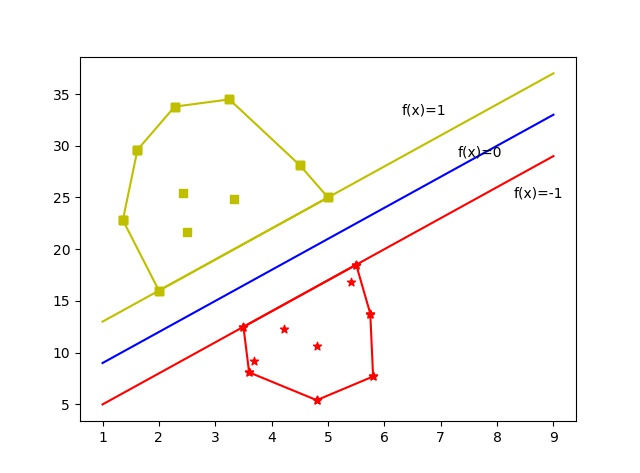
\includegraphics[width=9cm,height=6cm]{HullVector_SupportVector}
  \caption{Relationship between Convex-Concave Hull vectors and Support Vectors}
\end{figure}
Asdrúbal López Chau et al. $ ^{\cite{Asdrúbal López Chau et al.}}$ proposed convex-concave hull SVM classifier has distinctive advantages on dealing with large data sets with higher accuracy.As described in this paper, the vertices of the convex-concave hull are applied for SVM training with higher accuracy.In this work, a Convex-Concave Hull(CCH) SVM algorithm was used for classification due to its good incremental learning.

Now suppose that $X =\{x_{ij} | i = 1,2,...,c,j=1,2,...,N_i\}$ is the Raman spectrum data of  apple essences, where c is the apple essences class number, $x_{ij}$ represents the $j$th samples in class $i$,$N_i$ is the number of samples in class i. The overall apple essences sample size is N,which is expressed by
$$N = \sum _{i=1} ^{c} N_i$$

The Convex-Concave Hull of a set of points S is the minimum convex-concave set that contains S. Mathematically, CCH is defined as:
$$
CCH(X) :\{ \omega = \sum_{i=1} ^{n} \alpha_i x_i, \alpha_i \geq 0, \sum_{i=1} ^{n} = 1, x_i \in X \}
$$

Firstly, Let's create two subsets $X^+$ and $X^-$ from $X$
The procedure is summarized as follows, see Figure 2:
\begin{figure}[h]
  \centering
  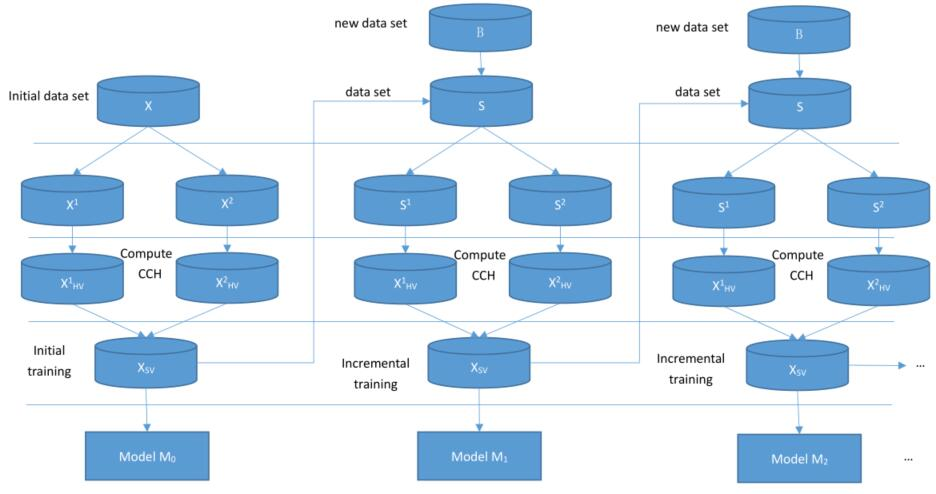
\includegraphics[width=9cm,height=6cm]{CCH-SVM}
  \caption{gneral process of CCH-SVM algorithm,take two classes as sample}
\end{figure}

\begin{enumerate}
\item Firstly,create subsets $X^i, i= 1,2,...,c$ from $X$.for each class data set $X^{i}$ , compute the Convex-Concave Hull vector set $X ^{i}_{H_{V}} = CCH(X_i)$, then make  $ X_{H_{V}} =X ^{1}_{H_{V}}  \bigcup X ^{2}_{H_{V}} \bigcup ...\bigcup X ^{c}_{H_{V}} $

\item Use $X_{H_{V}}$ as train data set, train SVM model,and get support vectors $X_{S_{V}}$

\item Add the incremental train data set S, splits into subsets $S^i ,( i= 1,2,...,c)$ from $S$.
make $X^i = S^i \bigcup X^i _{H_{V}}$ , compute the Convex-Concave Hull vector set $X ^{i}_{H_{V}} = CCH(X_i)$

\item As Convex-Concave Hull vector set $X_{H_{V}}$ as train data set to train SVM model,and get support vector set $X_{S_{V}}$ , then get the classifier.
Repeat steps 3) and 4) enable continuous incremental learning of new samples.
\end{enumerate}



%=============第三部分 数据分析===================
\section{Data Analysis}


% 拉曼数据分析

Raman spectrum can quickly obtain sample information about the functional groups in aromatic compounds,and has significant advantages that include simple sample preparation, rapid analysis, high sensitivity, robustness, green process, and low cost.

Since the Raman spectrum mainly reflected the main compounds of the essence, Raman spectrum of apple essences are extremely similar and difficult to be identified manually when the solvent of essences are the same. As shown in Figure 3. The spectrum of apple essences e, q, and s are similar while  i,a,c,d and f are similar..The spectrum B has more peaks,and contains the peaks of the previous two types of spectrum.According to the literature[23] and comparison of standards,the spectra of essences e, q, and s are mainly the peaks of 1,2-propanediol, and the spectra of essences  i,a,c,d and f are mainly the peaks of ethanol.

Raman  spectrum  of  essence samples  is  normally  very  complex  and  rich  of  chemical information.  Since  in essence  samples,  there  exist  different  types  of  functional group compound. The Raman spectrum of each of these compound consists of  numerous peaks.  The  visual  assignment  of  any  particular  peaks  to  a  specific  molecule usually  produces  imprecision  in  the  final  result,  because  most  of  the  time  different molecules  contribute  to  the  same  peak.  In  order  to  overcome  this  limitation  of  visual analysis, statistical methods are mostly used for the interpretation of Raman data of essence samples. With the statistical approach one can extract useful information from the data set by high  lighting  the  similarities  and differences.In  this  study,we  used Convex-Concave Hull SVM  for  the  classification of  apple essence,in order to efficiently handle large amounts of sample data.
%=============第四部分 结果与分析===================
\section{Result and Discussion}
% 实验结果
\subsection{Raw data of Characteristic Information}
% 拉曼光谱的三维图
\begin{figure}[h]
  \centering
  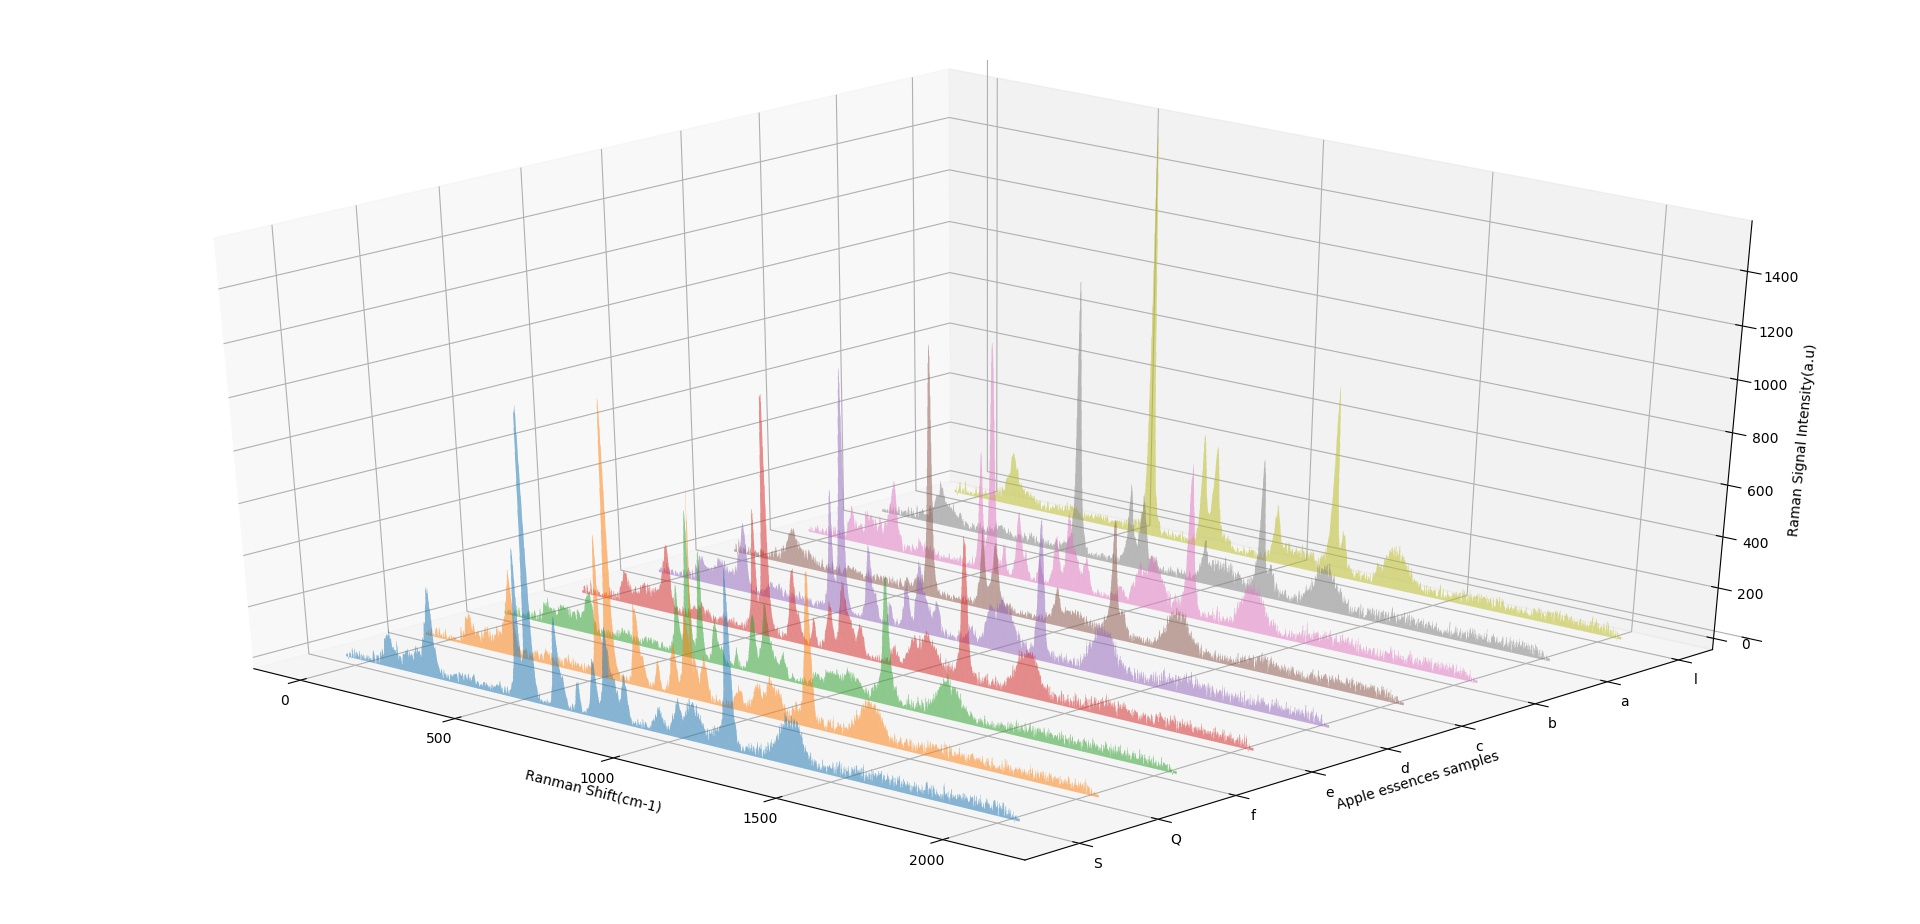
\includegraphics[width=9cm,height=6cm]{Typical_Raman_spectra}
  \caption{Typical Raman spectra of nine kinds of apple essences}
\end{figure}
Taking nine kinds of apple essences as example, figure x shows Raman spectra of apple essences.In the range of $1500 \sim 2350cm^{-1}$ band, the peak is small and mostly the background peak, so only the Raman spectral data in the $350 \sim 1500cm^{-1}$ band is considered for data processing. So the peak corresponding to $350 \sim 1500cm^{-1}$ band constitutes a feature vectors with the size of $ 1\times 1150 $.

%不同香精中化学成分及相对含量不尽相同,组分化合物间也会发生不同的缔合作用,
The chemical components and relative contents of different flavors are different, these will produce different associations, so it  determine the spectral curves of different flavors are somewhat different,and has different  characteristics and fingerprints. The difference between the spectra is the variation of relative intensities of the absorption peaks in the fingerprint region, and the minute difference in the small peaks in the fingerprint region. Pattern recognition algorithm can maximize the information extracted from the data, and can classify the sample set.


\subsection{Apple essences classification}
    \subsubsection{Data preprocessing results with PCA}

    \begin{figure}[h]
  \centering
  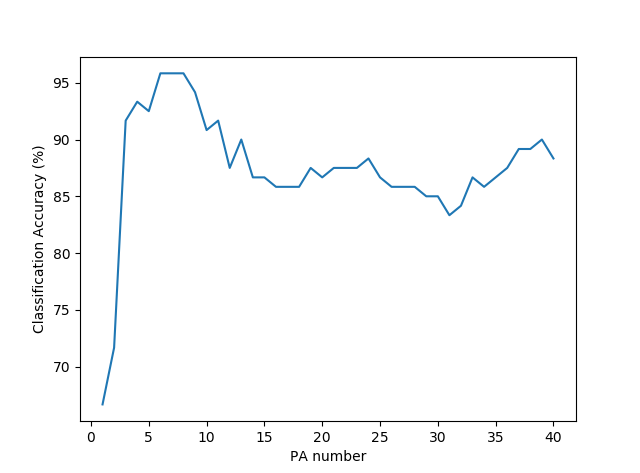
\includegraphics[width=10cm,height=6cm]{Figure_3}
  \caption{ The Classification rate of principal component number }
\end{figure}
Taking nine kinds of apple essences as example, figure x shows Raman spectra of apple essences. In the range of $1500 \sim  2350 cm^{-1}$ band, the peak is small and are mostly the background peak, so only the Raman spectral data in the $350 \sim 1500 cm^{-1}$ band is considered for data processing. So the peak corresponding to $ 350 \sim 1500 cm^{-1}$ band constitutes a feature vectors with the size of $ 1\times 1150 $.
The dimension of feature space generated by PCA is not determined by itself, and depended on the final classification rate and efficiency, according to Figure 4, We utilize 8 principal components as feature vectors, thinking of account the balance between efficiency and classification accuracy.

    \subsubsection{Classification result with CCH-SVM}

The CCH-SVM algorithm was used to classify the nine brands of apple essences samples. We selected the RBF kernel function in the CCH-SVM algorithm, and the kernel parameter was optimized using the Particle Swarm Optimization(PSO) method. To assess the performance of the established classifier, leave-one-out cross-validation and 10-fold cross-validation were conducted. These cross-validations fully assessed the performance of the classification model.
% CCH-SVM分类效果图


% 讨论分类效果


    \subsubsection{Compare data processing efficiency and accuracy}


% 对比不同方法的分类效果
For comparison, three different algorithms were simulated.Algorithm 1 uses the normal SVM algorithm, which uses all the samples to solve the support vector for each incremental learning. Algorithm 2 is SV-SVM algorithm, which uses the support vector set for incremental learning. Algorithm 3 is the CCH-SVM algorithm.The initial sample set is 100 samples randomly selected from all samples, and 16 samples are added for each incremental learning. The results are shown in Figure 5.

\begin{figure}[h]
  \centering
  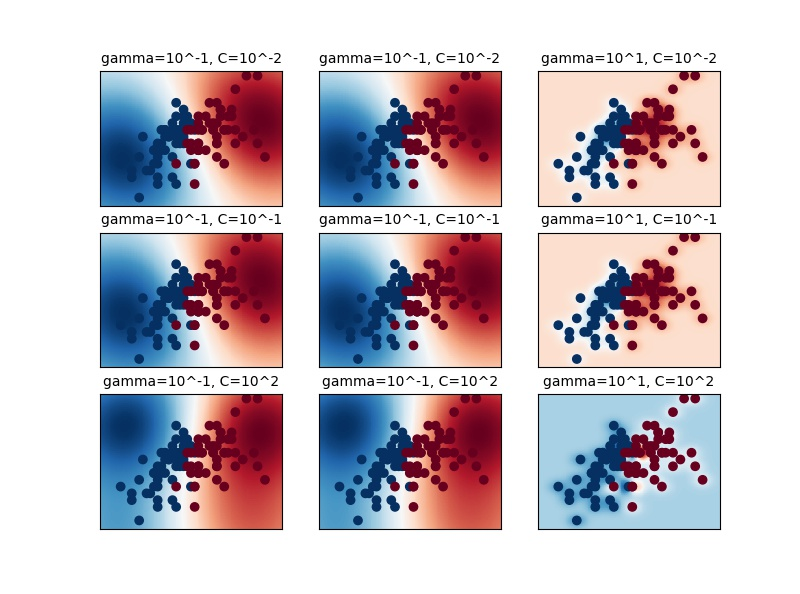
\includegraphics[width=15cm,height=6cm]{Figure_2}
  \caption{compare three algorithms}
\end{figure}

It can be seen from the simulation results that the CCH-SVM and SV-SVM incremental learning algorithm based on Convex-Concave Hull vector is compared with the standard SVM method, which greatly saves the computation time and accelerates the simulation speed, and the classification accuracy is basically the same, the algorithm, that combined the original support vector set with the new sample set rather than an initial sample set, greatly saves the computation time and accelerates the simulation speed, and the classification accuracy is basically the same.Meanwhile, with the continuous learning of incremental learning, the algorithm can naturally make part of the Convex-Concave Hull vector into non-Hull vector, to achieve the selective forgetting of the historical data of the training.Therefore, when dealing with a large number of new training data set ,the speed advantage of the incremental Convex-Concave Hull SVM method is more remarkable.

%=============第五部分 结论===================
\section{Conclusion}
This  study  demonstrates  the  use  of  Raman  spectrum  combined  with Convex-Concave-Hull SVM  technique  for the  classification  of  the  spectral  data  acquired  from  apple essences. Raman  spectroscopy  coupled  with  statistical  tools  has  great  potential  to  contribute significantly in the On-line inspection and research of product quality in an effective way.There is also a great  likelihood  to  use  Raman  spectroscopy  combined  with  one  of  the  existing  methods  for initial screening in order to increase the inspection efficiency. The results obtained are quite promising and interesting. The research work in our laboratory is still in progress striving for increasing sensitivity as well as specificity.

\section{Acknowledgements}
This paper was supported by the National Natural Science Foundation of China (No. 61373058).

\renewcommand\refname{References}
\begin{thebibliography}{30}
    % 苹果香精
    \bibitem{Sanz et al.}Sanz, C, Olias,  J.  M,  Perez,  A.  G. Aroma  bio-chemistry  of  fruits  and  vegetables.  In:  Tomas-Barberan,  F. A.; Robins, R. J. ed. Phytochemistryof  fruit  and  vegetables.  New  York,  Oxford  Uni-versity  Press  Inc.1997,125-155.
    \bibitem{K.P. Bennett1}K.P. Bennett , E.J. Bredensteiner, Geometry in Learning, Geometry at Work, C. Gorinieditors, Mathematical Association of America, 132-145, 2000
    \bibitem{K.P. Bennett2}K.P. Bennett , E.J. Bredensteiner, Duality and Geometry in SVM Classifiers, 17thInternational Conference on Machine Learning, San Francisco, CA, 2000
    %拉曼参考文献
    \bibitem{Zhou Xiu jun}Zhou Xiu jun,Dai Lian kui,Li Sheng.Fast Discrimination of Edible Vegetable Oil Based on Raman Spectroscopy.Spectroscopy and Spectral Analysis Spectrosc Spect Anal,2012,32(7):1829-1833
    \bibitem{WANG Jun}WANG Jun,ZHAO Yue-li.Application of Chromatogram Fingerprint in the Quality Controlof the Flavor and Perfume.NALYSIS AND TESTING TECHNOLOGY AND INSTRUMENTS,2005,11(3):192-196.
    \bibitem{SHA Min}SHA Min, SONG Chao, ZHANG Zhengyong et al.Discrimination of Apple Essences Based on Spectral Data Fusion Combined with Pattern Recognition Algorithm.FOOD SCIENCES,2016,37(22):192-197.
    % svm
    \bibitem{Vapnik}V.N. Vapnik, The Nature of Statistical Learning Theory, Springer, New York,1995, 8 (6) :988 - 999
    % 增量学习
    \bibitem{Stefan}Stefan Ruping,Incremental Learning with Support Vector Machines,Technical Reports,2001,228(4):641-642
    \bibitem{Asdrúbal López Chau et al.}Asdrúbal López Chau, Xiaoou Li, Wen Yu, Convex andconcave hulls for classification with support vector machine, Neurocomputing,http://dx.doi.org/10.1016/j.neucom.2013.05.040
    \bibitem{XIAORong}XIAO Rong, WANG Ji-cheng, SUN Zheng-xing. Anapproach to incremental SVM learning algorithm.Journal of Nanjing University, 2002, 38(2): 152 157.
    \bibitem{Zhu X}ZHU X, Lafferty J, Ghahramani Z. Combining active learning and semi-supervised learning using Gaussian fields  and  harmonic  functions[C].  In:  Proc  of  ICML  2003  Workshop  on  the  Continuum  from  Labeled  to Unlabeled Data. Menlo Park, CA:AAAI Press,2003:58-65.
    \bibitem{yunjungShin}Hyunjung Shin, Sungzoon Cho, Invariance of neighborhood relation underinput space to feature space mapping, Pattern Recognition Letters, 26 (2005)707–718.
    \bibitem{YJLee}Y.J. Lee, S.Y. Huang, Reduced support vector machines: a statistical theory,IEEE Transactions on Neural Networks 18 (No.1) (2007) 1–13.


\end{thebibliography}


\end{document}

